\chapter{مدل‌های پخشی و رویکرد‌های افزایش سرعت}
\section{تعاریف}
\subsection{مدل‌های مولد}

مدل‌های مولد عمیق دسته‌ای از مدل‌های پرکاربرد و جدید در حوزه‌ی هوش مصنوعی هستند که تلاش می‌کنند تا توزیع اصلی داده‌ی نمونه‌برداری شده را مدل کنند و با استفاده از این توزیع انواع مختلفی از سوالات در خصوص داده و دسته‌های آن را پاسخ دهند. در واقع اصلی‌ترین هدف یک مدل مولد، استفاده از مشاهدات شبیه‌سازی شده یا نمونه برداری شده از یک توزیع برای تخمین آن توزیع و سپس تولید نمونه‌های جدید از توزیع تخمین زده شده می‌باشد.
مدل‌های مولد کاربردهای متنوعی در یادگیری ماشین دارند، از جمله‌ی این کاربردها می‌توان به تولید عکس‌های باکیفیت، تولید قطعه‌های موسیقی و یا صوت، افزایش کارایی یادگیری نیمه نظارتی\LTRfootnote{Semi-supervised learning}، تشخیص ناهنجاری\LTRfootnote{Anomaly}، یادگیری تقلیدی و کمک به یادگیری تقویتی اشاره کرد. پیشرفت‌های اخیر این حوزه دو رویکرد کلی را دنبال می‌کنند: رویکردهای مبتنی بر درست‌نمایی\LTRfootnote{Likelihood} و شبکه‌های مولد تقابلی\LTRfootnote{Generative adversarial networks}. در رویکردهای مبتنی بر درست‌نمایی از لگاریتم درست‌نمایی یا خطاهای جایگزین به عنوان تابع هدف یادگیری استفاده می‌شود؛ در حالیکه در شبکه‌های مولد تقابلی تلاش می‌شود تا یادگیری با یک رویکرد تقابلی بین دو شبکه‌ی تمایزگر\LTRfootnote{Discriminatior} و تولیدکننده\LTRfootnote{Generator} صورت گیرد.
\\
با وجود عملکرد قابل توجه مدل‌های مبتنی بر درست‌نمایی وشبکه‌های مولد تقابلی، این مدل‌ها به واسطه‌ی نوع تعریفشان درگیر برخی محدودیت‌های ذاتی هستند. به عنوان مثال مدل‌های مبتنی بر درست‌نمایی برای ساخت توزیع‌های نرمال شده نیازمند به کارگیری معماری‌های خاص یا استفاده از توابع خطای جایگزین (مانند حد پایین مشاهده\LTRfootnote{Evidence lower bound} در خودکدگذارهای تغییراتی\LTRfootnote{Variational autoencoders}) در فرآیند یادگیری هستند. شبکه‌های مولد تقابلی مشکلات موجود در مدل‌های مبتنی بر درست‌نمایی را ندارند اما فرآیند یادگیری آنها به خاطر ماهیت تقابلی آن می‌تواند دچار ناپایداری شود. همچنین تابع هدف مدل‌های مولد تقابلی برای مقایسه و ارزیابی انواع این مدل‌ها چندان مناسب نیست\cite{song2019generative}.


\subsection{مدل‌های پخشی}
مدل‌های پخشی\LTRfootnote{Diffusion models} یک دسته‌ی نوظهور از مدل‌های مولد هستند که با توجه به عملکرد مناسب آنها در حوزه‌های تصویر، صوت، متن و گراف به سرعت مورد استقبال قرار گرفتند. وجه مشترک همه‌ی مدل‌های پخشی این است که در یک فرآیند رو به جلو\LTRfootnote{Forward process} داده را با نویز تخریب می‌کنند ودر نتیجه از توزیع داده به یک توزیع دلخواه قابل محاسبه می‌رسند و سپس در یک مسیر رو به عقب که توسط مدل یاد گرفته می‌شود، تلاش می‌کنند تا داده را بازسازی و از یک نمونه از توزیع دلخواه به یک نمونه از توزیع داده‌ها برسند. این موضوع درشکل \ref{diff} نشان داده شده است.
\\

\begin{figure}[!h]
	\begin{center}
		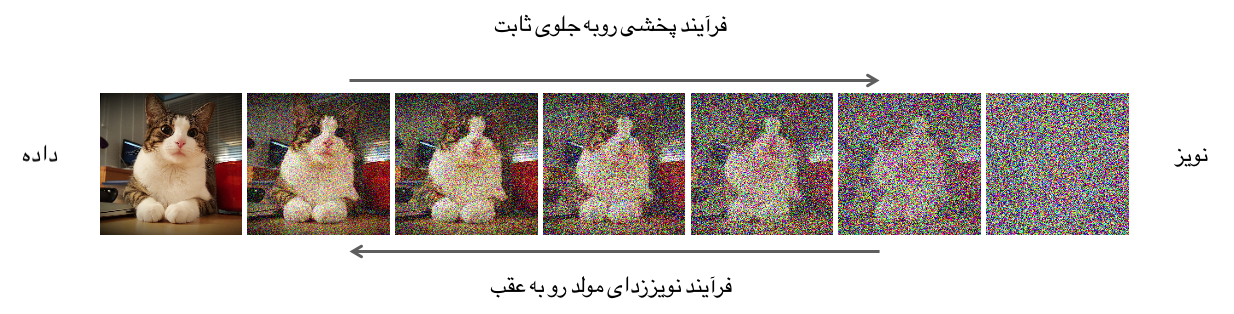
\includegraphics[width=15cm,height=4cm]{abstract.png}
		
		\caption{روند کلی یک مدل پخشی}
		\medskip
		\label{diff}
		\small
		در هر مدل پخشی یک فرآیند ثابت گام به گام رو به جلو برای تخریب داده و یک فرآیند معکوس برای تولید یک نمونه داده از نویز وجود دارد\cite{CiteDrive2022}.
	\end{center}
\end{figure}


با وجود اینکه چهارچوب گفته شده در بند قبل در همه‌ی مدل‌های پخشی وجود دارد؛ رویکردهای مختلفی برای فرموله سازی و پیاده سازی این روش وجود دارد. در مدل‌های مولد مبتنی بر تابع امتیاز\LTRfootnote{Score-based generative models} تلاش می‌شود با استفاده از گرادیان لگاریتم توزیع داده، که به آن تابع امتیاز\LTRfootnote{Score function} می‌گوییم، و یک فرآیند گام به گام حرکت در جهت این گرادیان نمونه‌ی جدید تولید کنیم. از طرفی در مدل‌های پخشی نویززدای احتمالاتی فرآیند تخریب داده و تولید نمونه با یک زنجیره‌ی مارکفی احتمالاتی مدل می‌شود و در نهایت در مدل‌های پخشی مبتنی بر معادلات دیفرانسیل تصادفی، فرآیند تخریب به صورت یک معادله دیفرانسیل تصادفی پیوسته مدل ‌می‌شود که با پیدا کردن معکوس این معادله و گسسته سازی آن امکان تولید نمونه‌ی جدید از توزیع داده‌ها فراهم می‌گردد.
\\
می‌توان نشان داد که مدل‌های پخشی بسیاری از محدودیت‌های مدل‌های مولد دیگر مانند نیاز به تمایزگر در شبکه‌های مولد تقابلی، نیاز به مقیدسازی شبکه در جریان‌های نرمال‌ساز\LTRfootnote{Normalizing flows} و نیاز به تنظیم توزیع‌های پسین در خودکدگذارهای تغییراتی را ندارند و قابلیت تولید تصاویر باکیفیت و متنوع را دارند. مشکل اصلی در مدل‌های پخشی فرآیند نمونه‌برداری طولانی آنهاست که باعث عدم کارایی این مدل‌ها در کاربردهای تعاملی می‌شود. با رفع این موضوع می‌توان اطمینان حاصل کرد که این دسته از مدل‌های مولد از توانایی همه‌جانبه‌ای برای به کارگیری در حوزه‌های مختلف برخوردار هستند.

\subsection{مدل‌های پخشی احتمالاتی نویززدا}


\subsubsection{تعریف مدل}
مدل‌های پخشی نویززدای احتمالاتی\LTRfootnote{Denoising diffusion probabilistic models(DDPMs)} یا به اختصار مپناها مدل‌هایی مبتنی بر متغیر پنهان\LTRfootnote{Latent variable models} هستند که از یک زنجیره‌ی مارکفی \LTRfootnote{Markov Chain}برای فرآیند پخشی استفاده می‌کنند. رویکرد کلی این مدل‌ها به این صورت است که در یک مسیر رو به جلو هر توزیع پیچیده‌ای از داده‌ها را می‌گیرد و آن را به یک توزیع اولیه که ساده و قابل محاسبه است تبدیل می‌کند و سپس یک مسیر روبه عقب محدود به زمان را یاد می‌گیرد که نمونه هایی از توزیع اولیه را به نمونه‌های توزیع داده تبدیل کند و این همان ایده‌ی کلی مدل مولد پخشی می‌باشد. تصویر \ref{ddpm1} این فرآیند را نشان می‌دهد. بنابراین این مدل سه مشخصه‌ی اصلی دارد: مسیر رو به جلو، مسیر رو به عقب و تابع مدل مولد که در ادامه هر یک را توضیح می‌دهیم.
\\
\begin{figure}[!h]
	\begin{center}
		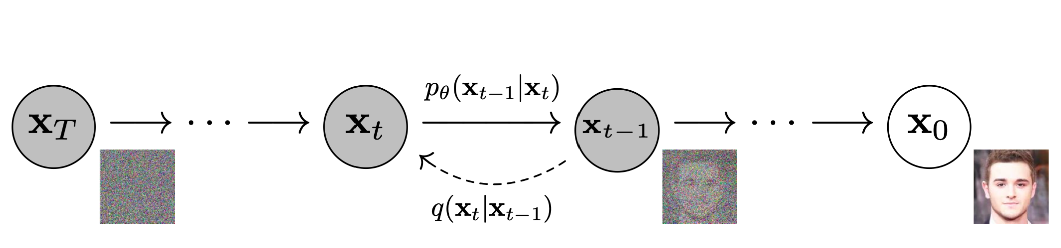
\includegraphics[width=15cm,height=4cm]{ddpm1.png}
		
		\caption{فرآیند پخش در مپناها}
		\medskip
		\label{ddpm1}
		\small
		مدل گرافی جهت‌دار یک مپنا که به صورت یک زنجیره‌ی مارکف روبه جلو و معکوس آن می‌باشد\cite{ho2020denoising}.
		
	\end{center}
\end{figure}


\subsubsection{مسیر رو به جلو}

اگر توزیع داده را با $q(x^{(0)})$ نشان دهیم، این توزیع به صورت مرحله به مرحله به یک توزیع $\pi(y)$ که از نظر آنالیزی قابل بیان است تبدیل می‌شود و این تبدیل توسط یک هسته‌ي $T_\pi(y|{y}’ ; \beta)$ صورت می‌گیرد که $\beta$ را نرخ پخش\LTRfootnote{Diffusion rate} می‌گوییم وداریم:

\begin{equation}
	\pi(y) = \int dy' \, T_\pi(y|y'; \beta) \pi(y')
\end{equation}

\begin{equation}
	q(x^{(t)} | x^{(t-1)}) = T_\pi(x^{(t)} | x^{(t-1)}}; \beta_t)
	\end{equation}
	
	و بنابراین مسیر رو به جلو\LTRfootnote{Forward trajectory} با شروع از توزیع داده ها و طی $T$ گام پخشی به صورت زیر است:
	
	\begin{equation}
q(x^{(0 \ldots T)}) = q(x^{(0)}) \prod_{t=1}^T q(x^{(t)}|x^{(t-1)})
\end{equation}

در ادامه‌ی این فصل هسته‌ی $ q(x^{(t)} | x^{(t-1)})$ هسته ی گاوسی در نظر گرفته می‌شود اما هسته‌های دیگری چون هسته‌ی دوجمله‌ای\LTRfootnote{Binomial kernel} نیز وجود دارند.
یک ویژگی حائز اهمیت مسیر رو به جلو این است که می‌توان به جای استفاده از فرم زنجیره‌ی مارکفی آن از یک فرم بسته استفاده کرد به این معنا که برای یافتن $x^{(t)}$ در زمان دلخواه $t$ می‌توان از رابطه‌ی زیر کمک گرفت:


\begin{equation}
q(x_t|x_0) = \mathcal{N}(x_t; \sqrt{\overline{\alpha}_t} x_0, (1 - \overline{\alpha}_t)I)
\end{equation}

که $ \overline{\alpha}_t := \prod_{s=1}^t \alpha_s$ و $ \alpha_t := 1 - \beta_t$ تعریف می‌شود.

\subsubsection{مسیر رو به عقب}

برای یادگیری توزیع مولد نیاز است که بتوانیم برعکس مسیر رو به جلو را یاد بگیریم و این به این معناست که باید بتوانیم از یک توزیع دلخواه قابل محاسبه به توزیع داده برسیم. بنابراین با تعریف توزیع اولیه به صورت $p(x^{(T)}) = \pi(x^{(T)})$ داریم:
\begin{equation}
p(x^{(0 \ldots T)}) = p(x^{(T)}) \prod_{t=1}^T p(x^{(t-1)}|x^{(t)})
\end{equation}
می‌توان نشان داد که اگر فرآیند پخش گاوسی باشد و گام‌های پخش $\beta$ خیلی کوچک باشند آنگاه معکوس فرآیند پخش نیز گاوسی می‌باشد\cite{feller2015retracted}. و بنابراین هر چقدر که طول این زنجیره بیشتر باشد $\beta$ کوچکتر می‌شود و می‌توان از تابع گاوسی برای مسیر معکوس نیز کمک گرفت. در فرآیند یادگیری با توجه به اینکه هسته‌ی گذر\LTRfootnote{Transition kernel} زنجیره ی مارکفی یک تابع گاوسی است، برای ساخت زنجیره تنها نیاز به میانگین و کوواریانس این تابع گاوسی داریم و در ادامه سعی می‌کنیم آنها را تخمین بزنیم.

\subsubsection{تابع مدل مولد}
تابع احتمال تولید شده توسط مپنا به صورت زیر می‌باشد:

\begin{equation}
p(x^{(0)}) = \int dx^{(1 \ldots T)} p(x^{(0 \ldots T)})
\end{equation}
از آنجاییکه انتگرال در حالت کلی غیرقابل محاسبه\LTRfootnote{Intractable} است، می‌‌توان با ایده گرفتن از نمونه برداری اهمیت\LTRfootnote{Importance sampling} به جای محاسبه‌ی انتگرال از میانگین احتمال نسبی مسیر رو به جلو و مسیر رو به عقب استفاده کرد که به صورت زیر قابل بیان است:



\begin{equation}
p(x^{(0)}) = \int dx^{(1 \ldots T)} q(x^{(1 \ldots T)}|x^{(0)}) \prod_{t=1}^T \frac{p(x^{(t-1)}|x^{(t)})}{q(x^{(t)}|x^{(t-1)})}
\end{equation}

\subsubsection{تعریف تابع خطا}
با توجه به مدل تعریف شده در قسمت قبل، آموزش شبکه معادل بیشینه کردن لگاریتم درست‌نمایی\LTRfootnote{Log-likelihood} تابع مدل مولد و یا کمینه کردن منفی این تابع است. بنابراین تابع هزینه را می‌توان به صورت زیر نوشت:


\begin{equation}
L = \int dx^{(0)} q(x^{(0)}) \log p(x^{(0)})
\end{equation}

در اینجا برای آموزش به جای بهینه سازی مستقیم لگاریتم درست‌نمایی از بهینه سازی حد تغییراتی\LTRfootnote{Variational bound} آن کمک می‌گیریم که به صورت زیر قابل تعریف است:

\begin{equation}
\label{vlb}
\mathbb{E}[-\log p_\theta(x^0)] \leq \mathbb{E}_q[-\log \frac{p_\theta(x^{0:T})}{q(x^{1:T}|x^0)}] = \mathbb{E}_q[-\log p(x^T) - \Sigma_{t \geq 1} \log \frac{p_\theta(x^{t-1}|x^{t})}{q(x^t|x^{t-1})}] =: L
\end{equation}

\subsubsection{تغییر پارامتر تابع خطا}
از آنجایی که ترکیب مسیر رو به جلو و مسیر معکوس شبیه به یک کدگذار تغییراتی است، می‌توان تابع هزینه را به صورت زیر بازنویسی کرد:

\begin{equation}
\label{total}
\mathcal{L}_{vlb} = \mathcal{L}_0 + \mathcal{L}_1 + \ldots + \mathcal{L}_{T-1} + \mathcal{L}_T
\end{equation}
\begin{equation}
\mathcal{L}_0 = -\log p_\theta(x_0|x_1)
\end{equation}
\begin{equation}
\label{lt1}
\mathcal{L}_{t-1} = \mathcal{D}_{KL}(q(x_{t-1}|x_t, x_0) \| p_\theta(x_{t-1}|x_t))
\end{equation}
\begin{equation}
\mathcal{L}_T = \mathcal{D}_{KL}(q(x_T|x_0) \| p(x_T))
\end{equation}

و از آنجایی که در صورت کوچک بودن $\beta_t$ هر دوی $ p_\theta(x_{t-1}|x_t))$ و $ q(x_{t-1}|x_t, x_0)$ توزیع هایی گاوسی هستند در نتیجه دیورجنس $KL$\LTRfootnote{KL-divergence} آنها را می‌توان به فرم تفاضل میانگین آنها در نظر گرفت و در نتیجه برای معادله ی (\ref{lt1})  داریم:

\begin{equation}
\label{lt2}
\mathcal{L}_{t-1} = \mathbb{E}_q \left[ \frac{1}{2\sigma_t^2} \|\tilde{\mu}_t(x_t, x_0) - \mu_\theta(x_t, t)\|^2 \right] + C
\end{equation} 

که در واقع نشان می‌دهد که در فرآیند آموزش یک مدل پخشی بهینه سازی خطا شامل تخمین میانگین پسین\LTRfootnote{Posterior mean} فرآیند رو به جلو می‌باشد. لازم است اشاره کنیم که در مقاله‌ی اصلی مقدار واریانس ثابت در نظر گرفته شده است. از طرفی با تغییر پارامتر $ x_t(x_0, \epsilon) = \sqrt{\bar{\alpha_t}}x_0 + \sqrt{(1 - \bar{\alpha_t})}\epsilon$ برای $ \epsilon \sim \mathcal{N}(0, I)$ و قراردهی آن در فرمول معادله‌ی (\ref{lt2}) می‌توان نشان داد که تخمین $\mu_\theta(x_t, t)$ به صورت زیر قابل پارامتری سازی است:

\begin{equation}
\mu_\theta(x_t, t) = \tilde{\mu}_t \left(x_t, \frac{1}{\sqrt{\bar\alpha_t}}\left(x_{t} - \sqrt{1-\bar\alpha_t}\epsilon_\theta(x_t)\right)\right) = \frac{1}{\sqrt{\alpha_t}} (x_t - \frac{\beta_t}{\sqrt{1 - \bar\alpha_t}}\epsilon_\theta(x_t, t)
\end{equation} 

که $\epsilon_\theta$ یک تخمین از نویز موجود در $x_t$ می‌باشد و در نتیجه برای محاسبه ی یک نمونه ی $x_{t-1}$ تنها کافیست که عبارت زیر را محاسبه کنیم:
\begin{equation}
\label{sample}
x_{t-1} = \frac{1}{\sqrt{\alpha_t}} (x_t - \frac{\beta_t}{\sqrt{1 - \bar\alpha_t}}\epsilon_\theta(x_t, t) + \sigma_tz
\end{equation}

که $z$ از توزیع گاوسی با میانگین صفر و کوواریانس همانی می‌ آید.

این تغییر پارامتر نشان می‌دهد که برای آموزش یک فرآیند رو به عقب می‌توان از تخمین $\tilde{\mu}_t$ با تابع میانگین وابسته به زمان $\mu_\theta$ استفاده کرد و یا مستقیما نویز اضافه شده به داده را با تخمین $\epsilon$ محاسبه کرد. 
\subsubsection{فرآیند یادگیری}
با توجه به تغییر پارامتر انجام شده در قسمت قبل و همچنین به کارگیری آن درمعادله‌ی ( \ref{total}) می توان به تابع هزینه ای رسید که کاملا نسبت به $\theta$ مشتق پذیر است و برای آموزش مناسب است اما برای سادگی پیاده سازی و افزایش کیفیت نمونه‌های تولیدی می‌توان تابع هزینه را به شکل زیر نیز بازنویسی کرد:

\begin{equation}
\label{loss}
L_{simple}(\theta) = \mathbb{E}_{t,x_0,\epsilon} \left[ \left \| \epsilon - \epsilon_\theta(\sqrt{\bar\alpha_t}x_0 + \sqrt{1-\bar\alpha_t}\epsilon, t) \right \|^2 \right]
\end{equation} 

که $t$ از یک توزیع یونیفرم بین ۱و $T$ می آید و واریانس $\beta_t$ در این فرآیند یک پارامتر ثابت بدون یادگیری می‌باشد. الگوریتم \ref{alg1} فرآیند آموزش یک مپنا را نشان می‌دهد.




% Algorithm 1: Training
\begin{algorithm}[H]
	\caption{آموزش}
	\begin{algorithmic}[1]
		\State مراحل زیر را تکرار کن
		\State $\mathbf{x}_0 \sim q(\mathbf{x}_0)$
		\State $t \sim \text{$Uniform$}(\{1, \ldots, T\})$
		\State $\boldsymbol{\epsilon} \sim \mathcal{N}(0, \mathbf{I})$
		\State گام نزول در جهت گرادیان را روی تابع زیر اعمال کن
		\[
		\nabla_\theta \|\boldsymbol{\epsilon} - \epsilon_\theta(\sqrt{\bar{\alpha}_t} \mathbf{x}_0 + \sqrt{1 - \bar{\alpha}_t} \boldsymbol{\epsilon}, t)\|^2
		\]
		\State تا زمانی که همگرا شود
	\end{algorithmic}
	\label{alg1}
\end{algorithm}

\subsubsection{فرآیند تولید نمونه‌ی جدید}
 همانطور که در الگوریتم \ref{alg2} نشان داده شده است؛ برای نمونه برداری ابتدا یک نمونه از توزیع  $\mathcal{N}(0, \mathbf{I})$ تولید می‌کنیم سپس به صورت معکوس هر بار نمونه را به شبکه می‌دهیم و نمونه‌ی نویززدایی شده را دریافت می‌کنیم. این فرآیند تا جایی ادامه پیدا می‌کند که به یک نمونه از توزیع $q(\mathbf{x}_0)$ برسیم.
 
 
% Algorithm 2: Sampling
\begin{algorithm}[H]
	\caption{نمونه‌برداری}
	\begin{algorithmic}[1]
		\State $\mathbf{x}_T \sim \mathcal{N}(0, \mathbf{I})$
		\State برای {$t = T, \ldots, 1$} مراحل زیر را انجام بده:
		\State $\mathbf{z} \sim \mathcal{N}(0, \mathbf{I})$ اگر $t > 1$، در غیر این صورت $\mathbf{z} = 0$
		\State $\mathbf{x}_{t-1} = \frac{1}{\sqrt{\alpha_t}} \left(\mathbf{x}_t - \frac{1 - \alpha_t}{\sqrt{1 - \bar{\alpha}_t}} \epsilon_\theta(\mathbf{x}_t, t)\right) + \sigma_t \mathbf{z}$
		\State پایان حلقه
		\State مقدار $\mathbf{x}_0$ را برگردان.
	\end{algorithmic}
	\label{alg2}
\end{algorithm}

در بخش بعدی سراغ انواع معماری‌ها و پیاده‌سازی‌های مپناها می‌رویم.


\subsection{انواع معماری مدل‌های پخشی نویززدای احتمالاتی}

در ساختار مپناها از هسته ی اصلی $pixelCNN++$ \cite{salimans2017pixelcnn++} استفاده شده است که در واقع نوعی شبکه‌ی یو با اتصالات گسترده‌ی باقی‌مانده‌ای می‌باشد. شکل\ref{ddpm2} ساختار کلی شبکه‌ی به کار گرفته شده را نشان می‌دهد.

\\
\begin{figure}[!h]
	\begin{center}
		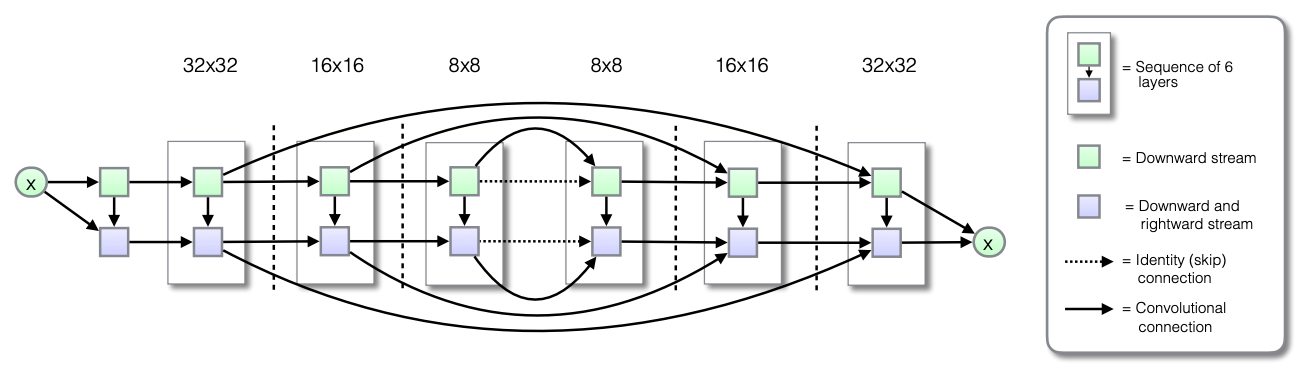
\includegraphics[width=15cm,height=5cm]{ddpm2.png}
		
		\caption{معماری $pixelCNN++$}
		\medskip
		\label{ddpm2}
		\small
		شبکه‌ی $pixelCNN++$ که نوعی شبکه‌ی یو با اتصالات باقی‌مانده‌ای گسترده است به عنوان شبکه‌ی اصلی در مپناها استفاده می‌شود\cite{salimans2017pixelcnn++}.
		
	\end{center}
\end{figure}

تا قبل از ارائه‌ی مدل پخشی نهان\LTRfootnote{Latent Diffusion model}\cite{rombach2022high}عمده‌ی ساختار ارائه شده برای مپنا به تنهایی بر پایه‌ی شبکه‌ی یو\cite{ronneberger2015u} یا یکی از انواع این شبکه بود. شبکه‌ی یو یک ساختار کدگذار-کدگشا\LTRfootnote{Encoder-Decoder} است که ابتدا برای مساله‌ی قطعه‌بندی تصاویر پزشکی ارائه شد. ویژگی خاص این شبکه‌ نسبت به سایر ساختار‌های کدگذار-کدگشا وجود اتصالات پرشی\LTRfootnote{Skip Connection} می‌باشد. این اتصالات با هدف ترکیب اطلاعات سطح بالا و اطلاعات محلی و نیز افزایش رزولوشن تصویر خروجی استفاده شدند. شکل \ref{unet} ساختار یک شبکه‌ی یو را نشان می‌دهد.

\begin{figure}[!h]
	\begin{center}
		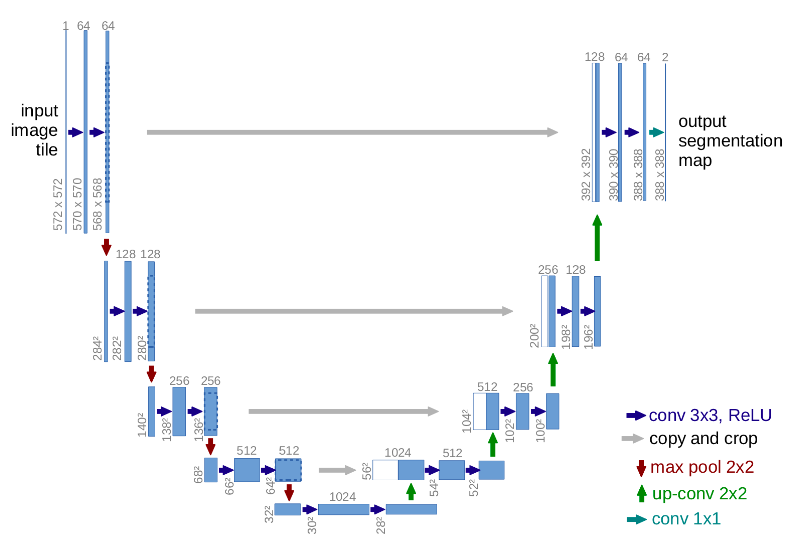
\includegraphics[width=15cm,height=10cm]{unet.png}
	\end{center}
	\caption{معماری شبکه‌ی یو}
	\medskip
	\label{unet}
	\small
	معماری کلی شبکه‌ی یو که اولین بار برای مساله‌ی قطعه‌بندی معنایی تصاویر پزشکی ارائه شد و شامل سه بخش کدگذار، کدگشا و اتصالات پرشی است\cite{ronneberger2015u}.
\end{figure}

\subsubsection{مدل پخشی نهان}
استفاده از شبکه‌ی یو به تنهایی، چالش‌های زیاد دارد؛ از جمله‌ی این مشکلات می‌توان به هزینه‌ی محاسباتی و سنگین بودن شبکه‌ی یو اشاره کرد که این موضوع با افزایش رزولوشن تصویر می‌تواند هزینه‌ی زیادی را ایجاد کند. از طرفی در اکثر مپناها فرآیند آموزش و نمونه‌برداری شبکه‌ی یو در فضای پیکسلی انجام می‌شود که مارا نیازمند تعریف یک شبکه‌ی متناظر به ازای هر رزولوشن و یا تغییر ابعاد تصویر می‌کند. علاوه بر موارد ذکر شده در شبکه‌های یوی به کار گرفته شده در فرآیند مپنا امکان شرطی‌سازی انعطاف پذیر وجود ندارد. این شبکه امکان انجام شرطی‌سازی بر اساس نام کلاس‌ها یا نویز ابتدایی تصویر را دارد ولی امکان دریافت متن و یا نقشه‌ی معنایی\LTRfootnote{Semantic Map} و پردازش آنها به عنوان شرط را بدون بهینه‌سازی در معماری ندارد.
\\
مدل‌های پخشی نهان با تمرکز بر رفع نقاط ضعف اشاره شده در مدل‌های شبکه‌ی یوی ابتدایی ارائه شدند. این مدل‌ها تلاش می‌کنند که اولا با انتقال تصویر از فضای پیکسلی به فضای پنهان با ابعاد کمتر از حجم محاسبات بکاهند. و ثانیا با اضافه کردن بلوک‌های توجه متقابل\LTRfootnote{Cross-Attention Blocks} انعطاف پذیری مدل‌ را به واسطه‌ی امکان شرطی‌سازی بر روی هر شکلی از شرط شامل متن یا نقشه‌ی معنایی افزایش دهند. خروجی این تغییرات باعث تولید تصاویر با کیفیت بهتر و در رزولوشن‌های بالاتر می‌باشد.
\\
شکل \ref{ldm} معماری این مدل را نشان می‌دهد. این مدل با به کارگیری یک خودکدگذار تغییراتی از پیش آموزش داده شده، ابتدا تصویر را از فضای پیکسلی به فضای پنهان می‌برد. در فضای پنهان، فرآیند یادگیری و نمونه‌برداری مشابه هر مدل مپنای دیگری انجام می‌شود و معماری اصلی شبکه‌ی نویززدا نیز یک شبکه‌ی یو با اتصالات پرشی و بلوک‌های توجه متقابل است. این مدل با استفاده از بلوک‌های توجه متقابل شرط را روی فرآیند نویززدایی اعمال می‌کند و در نهایت این مدل پس از پایان مراحل نویز زدایی تصویر را از فضای پنهان به فضای پیکسلی باز می‌گرداند.


\begin{figure}[!h]
	\begin{center}
		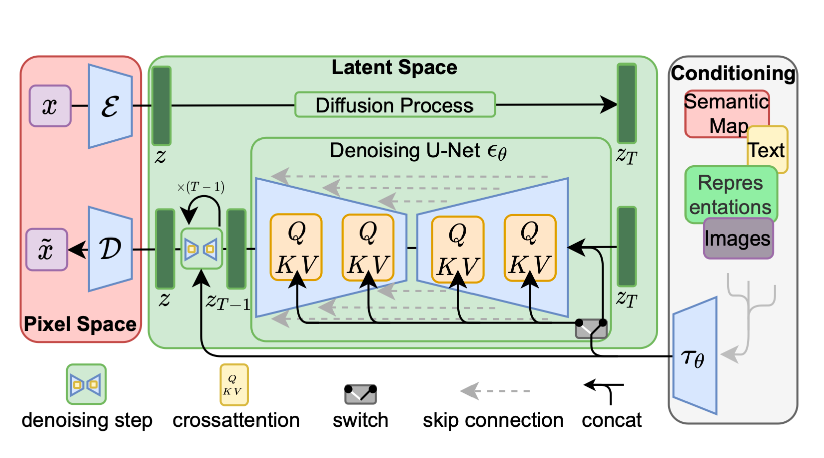
\includegraphics[width=15cm,height=8cm]{LDM.png}
	\end{center}
	\caption{معماری مدل‌های پخشی پنهان}
	\medskip
	\label{ldm}
	\small
	در شکل بالا شبکه‌ی $\epsilon$ کدگذار خود کدگذار تغییراتی است که تصویر ورودی $x$ را دریافت می‌کند و آن را به تصویر در فضای پنهان $z$ تبدیل می‌کند. همچنین $\tau_{\theta}$ یک کدگذار مختص دامنه‌ی مساله\LTRfootnote{Domain Specific Encoder} است که برای تبدیل شرط به یک بازنمایی قابل درک توسط مدل به کار گرفته می‌شود. همچنین $D$ نیز کدگشای خود کدگذار تغییراتی است که تصویر نویززدایی شده در فضای پنهان را به تصویر در فضای پیکسلی می‌برد\cite{rombach2022high}.
\end{figure}

مدل‌های $Diffusion$ $Stable$ که در این پروژه به کار گرفته شده اند؛ از این معماری تبعیت می‌کنند. که در فصل‌های  پیش رو در خصوص جزئیات پیاده‌سازی آنها بیشتر صحبت خواهیم کرد.

\subsubsection{مدل پخشی مبتی بر مبدل‌}

در مدل‌های پخشی مبتنی بر مبدل\LTRfootnote{Diffusion Transformer Models} \cite{peebles2023scalable}به جای استفاده از شبکه‌ی یو به عنوان شبکه‌ی نویززدا از ساختار مبدل تصویری\LTRfootnote{Vision Transformer} استفاده می‌شود. انتخاب این مبدل‌ها به عنوان هسته‌ی اصلی مدل‌های پخشی از این جهت است که هم می‌توانند وابستگی‌های\LTRfootnote{Long-range Dependency} قسمت‌های مختلف تصویر را مدل کنند و هم اینکه نسبت به شبکه‌ی یو ساختارهای مقیاس پذیرتری هستند. همچنین به کارگیری این مبدل‌ها در انواعی از دامنه‌ها مانند پردازش زبان طبیعی و سایر وظایف حوزه‌ی بینایی کارایی آنها را نسبت به سایر معماری‌ها نشان می‌دهد. و در نهایت وجود مکانیزم توجه به خود در مدل‌های مبدل باعث می‌شود که وابستگی‌های موجود در نواحی دور یا نزدیک تصویر به خوبی مدل می‌شوند.
\\
این مدل، مشابه مدل پخشی پنهان در فضای پنهان حاصل از یک خودکدگذار تغییراتی نویززدایی می‌کند. این مدل به جای استفاده از یک شبکه‌ی نویززدایی مبتنی بر شبکه‌ی یو از یک ساختار مطابق شکل \ref{} استفاده می‌کند. در این حالت ابتدا تصویر ورودی به فضای پنهان برده می‌شود و در آنجا مدل تصویر پنهان را به تعدادی قطعه\LTRfootnote{Patch} تقسیم می‌کند که توسط مبدل پردازش می‌شوند. همچنین در این مدل از یک رویکرد به نام $adaLN-zero$ برای اضافه کردن نام کلاس و شرطی‌سازی استفاده می‌شود. این رویکرد برخلاف مدل‌های پخشی پنهان که از یک بلوک توجه متقابل استفاده می‌کند، ابتدا شرط یا بازنمایی آن را از یک شبکه‌ی تماما متصل عبور می‌دهند و سپس آن را در قالب پارامتر‌های تغییر مقیاس\LTRfootnote{Scale Shift} به لایه‌های نرمالسازی لایه‌ای اضافه می‌کند.

\\
\begin{figure}[!h]
	\begin{center}
		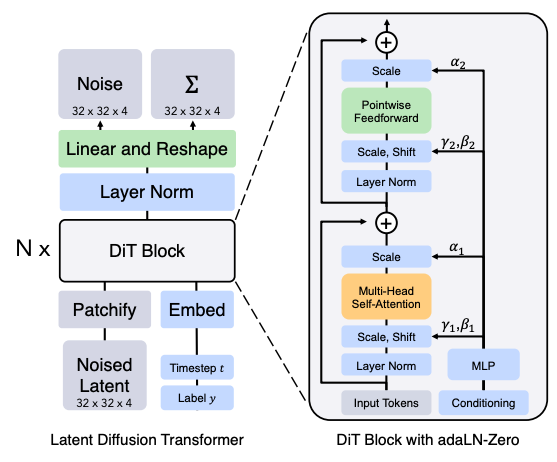
\includegraphics[width=10cm,height=9cm]{dit.png}
	\end{center}
	\caption{معماری مدل‌های مبتنی بر مبدل}
	\medskip
	\label{ldm}
	\small
		همانطور که شکل نشان ‌می‌دهد، ورودی‌های این مدل تصویر و زمان و برچسب کلاس هستند. تصویر ابتدا قطعه قطعه می‌شود و سپس وارد بلوک مبدل شده و در نهایت نیز یک تبدیل خطی روی آن انجام می‌شود تا با ترکیب قطعات مختلف تصویر نهایی ایجاد شود\cite{peebles2023scalable}.
\end{figure}

این مدل بر اساس اندازه‌ی قطعه، تعداد سر\LTRfootnote{Head}های مکانیزم توجه، تعداد لایه‌ها و اندازه‌ی لایه‌ی پنهان می‌تواند انواع گوناگونی داشته باشد. با توجه به آزمایشات انجام شده در مقاله مدل $DIT-XL$ با ۲۸ لایه، اندازه قطعه‌ی ۲، اندازه‌ی لایه‌ی پنهان ۱۱۵۲ و تعداد سرهای ۱۶ بهترین عملکرد را از خود ارائه می‌دهد.






